\section{Durchführung}
\label{sec:Durchführung}

\subsection{Einseitige Einspannung}

Zur Bestimmung des Elastizitätsmoduls wird eine Apparatur wie in \autoref{Abb:aufbau} verwendet. Es wird nacheinander ein Stab mit runder und quadratischer Grunfläche
wie in der Abbildung gezeigt am Punkt A eingespannt. Ein Gewicht kann nun am losen Ende des Stabes befestigt werden. Die Biegung des Stabes kann dann mit Hilfe der Messuhren
und der Längenskala an jedem Punkt in Form des vertikalen Abstandes zum Auflagepunkt gemessen werden. Da nicht davon auszugehen ist, dass er Stab vor Versuchsbeginn perfekt
gerade ist, wird zunächst eine Messung ohne Gewicht vorgenommen.
\begin{figure}
    \centering
    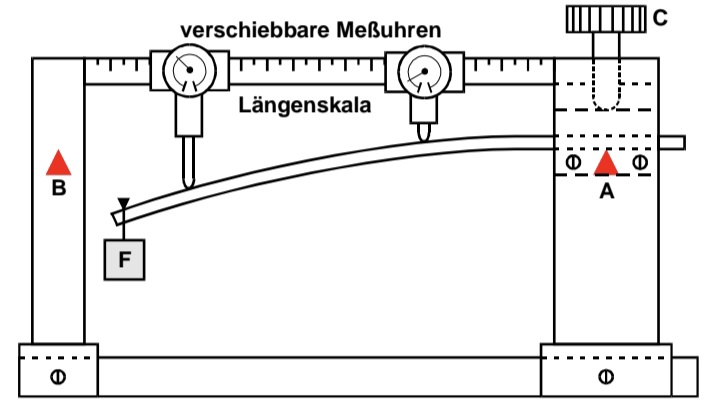
\includegraphics[width=5.5cm]{Dateien/v103Abbildung.jpg}
    \caption{Aufbau der verwendeten Messapparatur \cite{v103}.}
    \label{Abb:aufbau}
\end{figure}


\subsection{Beidseitige Auflage}
Im zweiten Teil der Messung werden die selben Stäbe nacheinander sowohl am Punkt A, als auch am Punkt B aufgelegt, jedoch ohne dabei eingespannt zu werden. Das Gewicht wird bei
diesem Aufbau in der Mitte des Stabes platziert, wobei auch hier zuvor eine Nullmessung ohne Gewicht vorgenommen wird. Die Messung der Biegung findet hierbei mit zwei verschiedenen Messuhren
statt, da durch das Gewicht in der Mitte eine durchgängige Messung mit einer Uhr nicht möglich ist.